%%%%%%%%%%%%%%%%%%%%%%%%%%%%%%%%%%%%%%%%%%%%%%%%%%%%%%%%%%%%%%%%%%%%%
%
%	Copyright 2014 Jean-Philippe Eisenbarth
%		Original template from:
%		https://github.com/Eisenbarth/SRS-Tex
%
%	Copyright 2016 Simone Bisi
%		Riadattato per il corso "Progetto del Software"
%		presso Università degli studi di Modena e Reggio Emilia
%
%		Progetto sviluppato entro 15gg dal 16 novembre 2016
%
%%%%%%%%%%%%%%%%%%%%%%%%%%%%%%%%%%%%%%%%%%%%%%%%%%%%%%%%%%%%%%%%%%%%%

\documentclass{scrreprt}

%%%%%%%%%%%%%%%%%%%%%%%%%%%%%%%%%%%%%%%%%%%%%%%%%%%%%%%%%%%%%%%%%%%%%

\usepackage{listings}
\usepackage{underscore}
\usepackage[bookmarks=true]{hyperref}
\usepackage[utf8]{inputenc}
\usepackage[italian]{babel}
\usepackage{afterpage}

\usepackage{makeidx}
\usepackage{hyperref}
\usepackage{bookmark}

\usepackage{placeins}
\usepackage{multirow}

\usepackage{fancyhdr}

\usepackage{graphicx}
\graphicspath{ {images/}}

%\usepackage{changepage}

\makeindex

%%%%%%%%%%%%%%%%%%%%%%%%%%%%%%%%%%%%%%%%%%%%%%%%%%%%%%%%%%%%%%%%%%%%%

\def \author 	{Simone Bisi}
\def \project 	{Software di gestione del\\personale aziendale}
\def \from		{Università degli studi di Modena\\e Reggio Emilia}

\hypersetup{
    bookmarks=false,    								% bookmarks
    pdftitle={Specifica dei requisiti del software},    % title
    pdfauthor={\author},	                     		% author
    pdfsubject={Gummi 0.6.5 and LaTeX},    				% subject
    pdfkeywords={}, 	% list of keywords
    colorlinks=true,    % false: boxed links; true: colored links
    linkcolor=blue,     % color of internal links
    citecolor=black,    % color of links to bibliography
    filecolor=black,    % color of file links
    urlcolor=purple,    % color of external links
    linktoc=page        % only page is linked
}
\date{}

%%%%%%%%%%%%%%%%%%%%%%%%%%%%%%%%%%%%%%%%%%%%%%%%%%%%%%%%%%%%%%%%%%%%%

\begin{document}

\begin{flushright}
    \rule{16cm}{5pt}\vskip1cm
    \begin{bfseries}
        \Huge{SPECIFICA DEI REQUISITI\\ DEL SOFTWARE}\\
        \vspace{1.9cm}
        per\\
        \vspace{1.9cm}
        {\normalfont{\textit{\project}}}
        \vspace{1.9cm}
        \LARGE{\textsc{ }}\\
        \vspace{1.9cm}
        di \author\\
        \vspace{0.5cm}
        \textsc{\from}\\
        \vspace{2.0cm}
        \today\\
    \end{bfseries}
\end{flushright}

%%%%%%%%%%%%%%%%%%%%%%%%%%%%%%%%%%%%%%%%%%%%%%%%%%%%%%%%%%%%%%%%%%%%%

\newcommand\blankpage{%
    \null
    \thispagestyle{empty}%
    \addtocounter{page}{-1}%
    \newpage}
    
\blankpage{}
\blankpage{}

%%%%%%%%%%%%%%%%%%%%%%%%%%%%%%%%%%%%%%%%%%%%%%%%%%%%%%%%%%%%%%%%%%%%%

\tableofcontents

%%%%%%%%%%%%%%%%%%%%%%%%%%%%%%%%%%%%%%%%%%%%%%%%%%%%%%%%%%%%%%%%%%%%%

\chapter{Introduzione}
%Introduzione globale all'intero SRS
La presente sezione ha lo scopo di riportare la visione globale dell'intero documento di specifica dei requisiti.
La struttura del documento è quella suggerita dallo standard ANSI/IEEE 830 noto come SRS (Software Requirements Spcifications).

%---------------------------------------------------------------------

\section{Obiettivo}
%Obiettivo del documento
%Utenza a cui è diretto
L'obiettivo del documento di specifica dei requisiti è quello di realizzare un software di gestione del personale di un'azienda.\\
Nello specifico, questo prodotto è diretto principalmente alla piccola e media impresa (\textit{PMI}, o \textit{SMB} nella sua connotazione anglosassone), ovvero aziende le cui dimensioni rientrano entro certi limiti occupazionali e finanziari prefissati. Non si esclude a priori l'utilizzo anche da parte di grandi aziende.\\
La specifica dei requisiti del sistema intende esprimere esclusivamente i bisogni informativi e di comunicazione, mentre le ipotesi sull'implementazione del prodotto verranno discusse nel documento di progettazione.

%---------------------------------------------------------------------

\section{Campo d'applicazione}
%Nome del prodotto da sviluppare
%Obiettivi del prodotto
%Principali benefici
%Problematiche che si intendono analizzare
%Problematiche che non saranno incluse nel processo di analisi
Il prodotto sviluppato prende il nome di \textit{EasyManage} e rappresenta un software per la gestione del personale aziendale.
\\
Nel dettaglio, si intende affrontare le problematiche di memorizzazione delle informazioni relative ai dipendenti di un'azienda e della gestione delle ore di straordinario effettuate da ogni dipendente nel corso del mese, in modo da poterle rendicontare allo stipendio di base definito dal contratto.
\\
Il software dovrà essere fruibile da tutti i dipendenti dell'azienda, pertanto dovrà essere sviluppato tenendo conto principalmente della semplicità d'uso e della sicurezza nella fase di accesso e di modifica dei dati personali.

\pagebreak

%---------------------------------------------------------------------

\section{Definizioni, acronimi, abbreviazioni}
%Definizione di tutti i termini utilizzati, acronimi e abbreviazioni

\FloatBarrier
\begin{table}[h|]
\centering
\begin{tabular}{|l|p{12cm}|}
\hline
\textbf{Entità} & \textbf{Definizione} \\ \hline
\textit{dipendente}  & { termine utilizzato per descrivere un qualsiasi membro del personale dell'azienda }                  \\ \hline
\textit{reparto}  & { settore dell'azienda specializzato in una determinata mansione }                  \\ \hline
\textit{operaio}  & { dipendente assegnato ad un certo reparto dell'azienda }                  \\ \hline
\textit{impiegato}  & { dipendente addetto alle mansioni di ufficio, tra cui il rendiconto degli stipendi dell'azienda }                  \\ \hline
\textit{capo reparto}  & { dipendente con mansioni simili a quelle dell'operaio, assegnato alla gestione di uno specifico reparto dal punto di vista amministrativo }                  \\ \hline
\textit{direttore}  & { proprietario o amministratore attuale dell'azienda }                  \\ \hline
\textit{stipendio base}  & { stipendio mensile di un dipendente come indicato sul contratto di assunzione }                  \\ \hline
\textit{straordinario}  & { ore lavorative di un dipendente oltre a quelle indicate sul contratto di assunzione }                  \\ \hline
\end{tabular}
\end{table}
\FloatBarrier

%---------------------------------------------------------------------

\section{Fonti}
%Elenco completo di tutte le fonti (documenti, libri, siti, altro)
Il documento è stato elaborato partendo dalle specifiche della traccia fornite dal docente Giacomo Cabri e completato con ipotesi ragionevoli per tutto ciò che non è specificato nel testo iniziale, di seguito riportato.
\begin{quote}
Progettare un sistema che possa essere utilizzato per gestire il seguente dominio applicativo. Una azienda
ha un certo numero di dipendenti, divisi tra operai e impiegati; ogni dipendente appartiene ad un livello di
anzianità. Gli operai sono divisi in reparti e ogni reparto ha un capo reparto. Gli impiegati invece dipendono
dal direttore generale. Ogni operaio può effettuare delle ore di straordinario, sia su sua richiesta
autorizzata dal capo reparto, sia su richiesta del capo reparto o del direttore generale. Allo stesso modo gli
impiegati possono effettuare ore di straordinario su propria richiesta autorizzata dal direttore generale o
richieste dal direttore generale stesso.\\
Gli impiegati devono gestire tutti gli aspetti relativi allo stipendio, conteggiando lo stipendio di partenza in
base al livello di ogni dipendente e aggiungendo le ore di straordinario effettuate. Ogni dipendente può
vedere la propria situazione oraria ma non modificarla. Ogni capo reparto può vedere la situazione oraria di
tutti gli operai del suo reparto. Gli impegati possono vedere e modificare la situazione di qualsiasi
dipendente.
\end{quote}
Il documento è stato realizzato mediante l'utilizzo del linguaggio di markup \LaTeX\\ e compilato in PDF mediante l'editor \textit{Gummi}.

%---------------------------------------------------------------------

\pagebreak

\section{Struttura del documento}
%Organizzazione del documento delle specifiche
Il documento è diviso in varie sezioni, già specificate nell'indice di testa.

\FloatBarrier
\begin{table}[h|]
\centering
\begin{tabular}{|l|l|p{10cm}|}
\hline
 & \textbf{Sezione} & \textbf{Funzione} \\ \hline
1 & \textit{Introduzione} & Presenta il prodotto soggetto alla specifica dei requisiti e si illustrano eventuali termini ricorrenti \\ \hline
2 & \textit{Descrizione generale} & Si cerca di inquadrare il più possibile gli utilizzatori finali del software \\ \hline
3 & \textit{Specifica dei requisiti} & Espone i requisiti funzionali e non funzionali necessari ad implementare il software \\ \hline
4 & \textit{Diagrammi} & Si mostrano i diagrammi dei casi d'uso, delle attività e delle classi \\ \hline
5 & \textit{Design Patterns} & Si individuano design patterns per facilitare la fase di progettazione del software \\ \hline
\end{tabular}
\end{table}
\FloatBarrier

%%%%%%%%%%%%%%%%%%%%%%%%%%%%%%%%%%%%%%%%%%%%%%%%%%%%%%%%%%%%%%%%%%%%%

\chapter{Descrizione generale}
%Principali fattori che riguardano il prodotto e i suoi requisiti
%Regole fondamentali per il concreto funzionamento del prodotto e per
%il soddisfacimento dei requisiti (sezione 3)
%Non ci sono ancora requisiti veri e propri
Questa sezione evidenzia i principali fattori che riguardano il prodotto ed i requisiti fondamentali per il suo concreto funzionamento.

%---------------------------------------------------------------------

\section{Inquadramento}
\label{sec:inquadramento}
%Confronto del sistema con altri prodotti simili
Il prodotto sviluppato si propone come soluzione per la gestione aziendale dell'assegnazione delle ore di straordinario dei dipendenti e di calcolo del loro stipendio mensile.

	\subsection{Interfaccia di sistema}
	%Caratteristiche dell'interfaccia con il sistema
	Il prodotto viene sviluppato tramite linguaggi e framework che ne consentano la portabilità tra i principali sistemi operativi disponibili in commercio (Windows, macOS, Linux) se necessario.

	\subsection{Interfaccia utente}
	%Caratteristiche dell'interfaccia con l'utente
	%In termini di formato dello screen, layout di pagine, contenuti
	%del report o dei menù, lunghezza messaggi di errore
	Il prodotto risulta dotato di un'interfaccia utente (GUI) chiara ed efficace, che non richiede formazione specifica del personale per l'utilizzo. L'interfaccia grafica si adatta alla maggior parte delle risoluzioni disponibili (grazie all'utilizzo di soluzioni già testate di tipo free o \textit{Commercial Off-The-Shelf}) sul mercato e cerca di essere il più possibile chiara per l'utente finale tramite l'utilizzo di icone univoche ed intuitive.

	\subsection{Interfaccia hardware}
	%Informazioni per configurare adeguatamente il sistema
	Il prodotto non richiede l'installazione di hardware specifici. Si suppone che il cliente disponga quanto meno di un elaboratore con i requisiti minimi per il funzionamento dei principali sistemi operativi moderni.

	\subsection{Interfaccia software}
	%Eventuale necessità d'uso di altri pacchetti software di 
	%supporto
	%Interlacciamento con altre applicazioni
	Il prodotto viene distribuito come applicativo \textit{stand-alone}, ovvero capace di funzionare da solo e in maniera indipendente da altri oggetti o software, con cui potrebbe altrimenti interagire.

	\subsection{Interfaccia di comunicazione}
	%Protocolli di comunicazione (TCP/IP)
	Il prodotto non necessita di accesso ad Internet e di comunicare con reti esterne all'azienda.

	\subsection{Vincoli di occupazione di memoria}
	%Caratteristiche e limiti dei supporti di memoria
	%primaria e secondaria
	Il prodotto compilato ha una dimensione irrisoria, sia nel supporto di memorizzazione secondaria che in fase di esecuzione in quella primaria.

	\subsection{Operazioni}
	%Operazioni di inizializzazione, backup e recovery del sistema
	Il prodotto non deve eseguire operazioni di inizializzazione al suo avvio e non esegue autonomamente operazioni di backup e recovery.

	\subsection{Vincoli di installazione}
	%Vincoli per ciascun nodo (es. sequenza inizializzazione, livello
	%di sicurezza richiesto, ...)
	L'installazione del prodotto richiede l'autenticazione al sistema operativo come utente autorizzato ad installare software sulla macchina.

%---------------------------------------------------------------------

\section{Funzioni del prodotto}
%Principali funzionalità, elencate a grandi linee
Il prodotto è indirizzato a mantenere un database di informazioni relative ai dipendenti dell'azienda e di gestire gli stipendi dei dipendenti in funzione delle ore di straordinario effettuate da questi ultimi (volontariamente o su richiesta specifica di un superiore).

%---------------------------------------------------------------------

\section{Caratteristiche degli utenti finali}
%Caratteristiche degli utenti del sistema in termini di esperienza,
%capacità tecnica e livello di istruzione
Si delineano quattro categorie di utenti finali: \textit{impiegato, operaio, direttore, capo reparto}. Tutti gli utenti finali devono possedere competenze di base per l'utilizzo di un computer. Gli impiegati, incaricati di gestire tutti gli aspetti relativi allo stipendio, devono essere a conoscenza dei metodi di retribuzione applicati dall'azienda nei confronti dei propri dipendenti.\\
Gli operai individuano come superiori il proprio capo reparto ed il direttore. Gli impiegati ed i capi reparto individuano come superiori il direttore.\\
Per comodità progettuale tutte le persone che effettivamente lavorano nell'azienda, direttore compreso, vengono registrate come \textit{Membro}. Tutti coloro che sono risultano sottoposte al direttore vengono registrate come \textit{Dipendente}.\\
Non si richiede ulteriore esperienza o capacità tecnica per l'esecuzione del software.

%---------------------------------------------------------------------

\section{Vincoli generali}
%Vincoli che verranno affrontati durante lo sviluppo (interfacciamento
%con altri sistemi, operazioni parallele, elementi di criticità)
Non si individuano vincoli particolari di interfacciamento con altri sistemi, operazioni parallele o elementi di criticità.

%---------------------------------------------------------------------

\section{Ipotesi iniziali}
%Ipotesi di partenza, assunzioni e dipendenze
%Fattori che, eventualmente modificati, hanno ripercussioni sul 
%contenuto dell'SRS
L'amministratore di sistema fornisce le credenziali per i dipendenti, ovvero ID e password iniziale generata casualmente. Si suppone che al momento dell'assunzione i dipendenti ottengano le informazioni necessarie per accedere al sistema, analogamente ai dipendenti già assunti nell'azienda.\\
Si suppone che esista attualmente un registro (cartaceo o su altro supporto) che permetta agli impiegati di trasferire i dati nel nuovo software.

%---------------------------------------------------------------------

\section{Requisiti futuri}
%Requisiti che verranno dettagliati in futuro (meglio specificare
%quando e da chi)
Si deve prevedere nello sviluppo del software la possibilità di modificare, aggiungere o rimuovere in modo agevole nuove tipologie di dipendenti tramite una metodologia di sviluppo modulare.\\
Sarà necessario inoltre verificare la reale affidabilità del prodotto nel breve e lungo periodo su diverse aziende campione, la soddisfazione dei clienti ed il grado di semplicità con cui gli utilizzatori del software si ritrovano nell'interfaccia grafica.

%%%%%%%%%%%%%%%%%%%%%%%%%%%%%%%%%%%%%%%%%%%%%%%%%%%%%%%%%%%%%%%%%%%%%

\chapter{Specifica dei requisiti}
%Sezione principale, riporta i requisiti funzionali e non funzionali
La sezione di specifica dei requisiti è la parte principale del documento e riporta tutti i requisiti del prodotto, divisi nelle categorie \textit{funzionali} e \textit{non funzionali}.

%---------------------------------------------------------------------

\section{Requisiti dell'interfaccia esterna}
%Specifica l'interfaccia del software verso l'esterno (I/O)
%Complementare alle specifiche in 2.1 (Inquadramento)
Si ritengono descritti sufficientemente i dettagli riguardanti l'interfaccia del software verso l'esterno nella sezione \hyperref[sec:inquadramento]{\textit{2.1}}. 

%---------------------------------------------------------------------

\section{Requisiti funzionali}
%Ogni requisito è descritto tramite una scheda/tabella
%
%	- introduzione
%		> attori coinvolti
%		> descrizione generale della funzione
%	- input
%		(informazioni che sono gestite all'interno del processo
%		come ingresso)
%		> descrizione generica dei dati
%	- descrizione (processo)
%		(sequenza di azioni eseguite dall'operatore, eventuali
%		messaggi di errore come risposta ad anomalie e parametri
%		che incidono sull'output)
%		> validazione dei dati
%		> sequenza di operazioni
%		> risposta ad eventuali anomalie
%		> parametri che impattano sull'output
%	- output
%		(risultato del processo)
%
%	(tabella alternativa)
%	----------------------------------------------------
%	Codice 		| Area di riferimento | Titolo specifico
%	----------------------------------------------------
%	Input  		|
%	----------------------------------------------------
%	Descrizione |
%	(processo)  |
%	----------------------------------------------------
%	Output		|
%	----------------------------------------------------
%

\newcounter{rfu}
\stepcounter{rfu}

I requisiti funzionali descrivono come il sistema deve comportarsi in base agli input degli utenti finali e nelle varie situazioni d'uso.

\newcommand{\specialcell}[2][c]{%
  \begin{tabular}[#1]{@{}l@{}}#2\end{tabular}}

%... Visualizza stato
\begin{table}[h|]
\centering
\begin{tabular}{|l|p{6cm}|p{6cm}|}
\hline
\textbf{RF\therfu} & \textbf{Operazioni di gestione} & \textbf{Visualizzazione di un dipendente} \\ \hline
Attori & \multicolumn{2}{p{12cm}|}{ Membro } \\ \hline
Input  & \multicolumn{2}{p{12cm}|}{ \specialcell{ID del dipendente\\Password del dipendente} }                  \\ \hline
Descrizione  & \multicolumn{2}{p{12cm}|}{Un qualsiasi membro dell'azienda accede al sistema tramite il proprio ID e la propria password. Se questi risultano corretti si accede alla propria scheda.}                  \\ \hline
Output  & \multicolumn{2}{p{12cm}|}{ \specialcell{Informazioni base della scheda dipendente\\
Eventuali informazioni riguardanti ore di straordinario assegnate} }                  \\ \hline
\end{tabular}
\end{table}
\stepcounter{rfu}

%... Modifica stato
\begin{table}[h|]
\centering
\begin{tabular}{|l|p{6cm}|p{6cm}|}
\hline
\textbf{RF\therfu} & \textbf{Operazioni di gestione} & \textbf{Modifica stato di un dipendente} \\ \hline
Attori & \multicolumn{2}{p{12cm}|}{ \specialcell{Impiegato, Dipendente} } \\ \hline
Input  & \multicolumn{2}{p{12cm}|}{
\specialcell{ID del dipendente\\Modifiche alla scheda del dipendente} }                  \\ \hline
Descrizione  & \multicolumn{2}{p{12cm}|}{Un impiegato seleziona il dipendente da modificare da un apposito form ed ottiene la visualizzazione della scheda dipendente attuale. Da lì può operare sui valori modificabili (anagrafica, stipendio, ore di straordinario, ...), senza poter modificare altri valori (ID del dipendente). Dopo aver completato le modifiche può salvare il form o annullare e tornare alla pagina precedente.}                  \\ \hline
Output  & \multicolumn{2}{p{12cm}|}{ \specialcell{Visualizzazione della scheda del dipendente dopo le modifiche} }                  \\ \hline
\end{tabular}
\end{table}
\stepcounter{rfu}

%... Richiede straordinario

\begin{table}[h|]
\centering
\begin{tabular}{|l|p{6cm}|p{6cm}|}
\hline
\textbf{RF\therfu} & \textbf{Ore di straordinario} & \textbf{Richiesta straordinario} \\ \hline
Attori & \multicolumn{2}{p{12cm}|}{ Dipendente, Direttore } \\ \hline
Input  & \multicolumn{2}{p{12cm}|}{ \specialcell{Data\\Numero di ore\\Motivazione (opzionale)} }                  \\ \hline
Descrizione  & \multicolumn{2}{p{12cm}|}{Il dipendente inserisce una richiesta per effettuare ore di straordinario destinata al direttore}                  \\ \hline
Output  & \multicolumn{2}{p{12cm}|}{Conferma dell'inserimento della richiesta}                  \\ \hline
\end{tabular}
\end{table}
\stepcounter{rfu}

%... Ordine straordinario
\begin{table}[h|]
\centering
\begin{tabular}{|l|p{6cm}|p{6cm}|}
\hline
\textbf{RF\therfu} & \textbf{Ore di straordinario} & \textbf{Ordine straordinario} \\ \hline
Attori & \multicolumn{2}{p{12cm}|}{Direttore, Dipendente} \\ \hline
Input  & \multicolumn{2}{p{12cm}|}{\specialcell{Data\\Numero di ore\\Motivazione (opzionale)\\ID del dipendente}}                  \\ \hline
Descrizione  & \multicolumn{2}{p{12cm}|}{Il direttore inserisce una richiesta per effettuare ore di straordinario destinata ad un dipendente.}                  \\ \hline
Output  & \multicolumn{2}{p{12cm}|}{Conferma dell'inserimento dell'ordine}                  \\ \hline
\end{tabular}
\end{table}
\stepcounter{rfu}

%... Valuta straordinario
\begin{table}[h|]
\centering
\begin{tabular}{|l|p{6cm}|p{6cm}|}
\hline
\textbf{RF\therfu} & \textbf{Ore di straordinario} & \textbf{Valuta straordinario} \\ \hline
Attori & \multicolumn{2}{p{12cm}|}{Direttore, Dipendente} \\ \hline
Input  & \multicolumn{2}{p{12cm}|}{\specialcell{Richiesta di un dipendente\\Scelta riguardo la richiesta}}                  \\ \hline
Descrizione  & \multicolumn{2}{p{12cm}|}{Il direttore valuta una richiesta per effettuare ore di straordinario di un dipendente in modo positivo o negativo.}                  \\ \hline
Output  & \multicolumn{2}{p{12cm}|}{Conferma della valutazione}                  \\ \hline
\end{tabular}
\end{table}
\stepcounter{rfu}

%... Richiesta straordinario (reparto)
\FloatBarrier
\begin{table}[h|]
\centering
\begin{tabular}{|l|p{6cm}|p{6cm}|}
\hline
\textbf{RF\therfu} & \textbf{Ore di straordinario} & \textbf{\specialcell{Richiesta straordinario\\(reparto)}} \\ \hline
Attori & \multicolumn{2}{p{12cm}|}{ Operaio, Capo Reparto } \\ \hline
Input  & \multicolumn{2}{p{12cm}|}{ \specialcell{Data\\Numero di ore\\Motivazione (opzionale)} }                  \\ \hline
Descrizione  & \multicolumn{2}{p{12cm}|}{L'operaio inserisce una richiesta per effettuare ore di straordinario destinata al capo del proprio reparto operativo in azienda}                  \\ \hline
Output  & \multicolumn{2}{p{12cm}|}{Conferma dell'inserimento della richiesta}                  \\ \hline
\end{tabular}
\end{table}
\stepcounter{rfu}
\FloatBarrier

%... Ordine straordinario (reparto)
\begin{table}[h|]
\centering
\begin{tabular}{|l|p{6cm}|p{6cm}|}
\hline
\textbf{RF\therfu} & \textbf{Ore di straordinario} & \textbf{\specialcell{Ordine straordinario\\(reparto)}} \\ \hline
Attori & \multicolumn{2}{p{12cm}|}{Capo reparto, operaio} \\ \hline
Input  & \multicolumn{2}{p{12cm}|}{\specialcell{Data\\Numero di ore\\Motivazione (opzionale)\\ID dell'operaio}}                  \\ \hline
Descrizione  & \multicolumn{2}{p{12cm}|}{Il capo reparto inserisce una richiesta per effettuare ore di straordinario destinata ad un operaio che lavora nel suo reparto di competenza.}                  \\ \hline
Output  & \multicolumn{2}{p{12cm}|}{Conferma dell'inserimento dell'ordine}                  \\ \hline
\end{tabular}
\end{table}
\FloatBarrier
\stepcounter{rfu}

%... Valuta straordinario
\begin{table}[h|]
\centering
\begin{tabular}{|l|p{6cm}|p{6cm}|}
\hline
\textbf{RF\therfu} & \textbf{Ore di straordinario} & \textbf{Valuta straordinario (reparto)} \\ \hline
Attori & \multicolumn{2}{p{12cm}|}{Capo Reparto, Operaio} \\ \hline
Input  & \multicolumn{2}{p{12cm}|}{\specialcell{Richiesta di un dipendente\\Scelta riguardo la richiesta}}                  \\ \hline
Descrizione  & \multicolumn{2}{p{12cm}|}{Il capo reparto valuta una richiesta per effettuare ore di straordinario di un operaio in modo positivo o negativo.}                  \\ \hline
Output  & \multicolumn{2}{p{12cm}|}{Conferma della valutazione}                  \\ \hline
\end{tabular}
\end{table}
\stepcounter{rfu}

\pagebreak

%---------------------------------------------------------------------

\section{Requisiti non funzionali}
I requisiti non funzionali descrivono le proprietà e le qualità dei servizi offerti dal sistema in maniera quantificabile.

\newcounter{rnf}
\stepcounter{rnf}

	\subsection{Requisiti prestazionali}
	%Numero di terminali supportati
	%Numero di utenti che hanno accesso al sistema contemporaneamente
	%Quantità e tipo di informazioni che possono essere manipolate
	%contemporaneamente
	
	%.............................................................
	
	\FloatBarrier
	\begin{table}[h|]
	\centering
	\begin{tabular}{|l|p{6cm}|p{6cm}|}
	\hline
	\textbf{RNF\thernf} & \textbf{Requisiti prestazionali} & \textbf{Tempi di risposta} \\ \hline
	Descrizione  & \multicolumn{2}{p{12cm}|}{ Il software deve avere tempi di risposta rapidi. Oltre alla prestazione computazionale della macchina, non è necessario tenere conto di ulteriori fattori di rallentamento. Ci si aspetta di ottenere tempi di risposta nell'ordine di 1 secondo nel 95\% dei casi, mentre nel restante 5\% non si devono superare i 5 secondi. }                  \\ \hline
	\end{tabular}
	\end{table}
	\FloatBarrier
	\stepcounter{rnf}

	%.............................................................

	\subsection{Database}
	%Tipo di database che si intende utilizzare
	%Database non compatibili con le caratteristiche del prodotto
	\FloatBarrier
		\begin{table}[h|]
	\centering
	\begin{tabular}{|l|p{6cm}|p{6cm}|}
	\hline
	\textbf{RNF\thernf} & \textbf{Database} & \textbf{Gestione dei dati} \\ \hline
	Descrizione  & \multicolumn{2}{p{12cm}|}{Il software viene sviluppato in relazione ad un particolare DBMS (Data Base Management System) in fase di progettazione. Si individuerà un DBMS presente sul mercato con licenza d'uso \textit{free/FOSS} che verrà configurato automaticamente durante l'installazione del prodotto. I dati di accesso al database vengono resi noti esclusivamente all'amministratore di sistema. }                  \\ \hline
	\end{tabular}
	\end{table}
	\FloatBarrier
	\stepcounter{rnf}

	%.............................................................

	\subsection{Vincoli generali di progetto}
	%Vincoli imposti da altri standard
	%Limitazioni hardware
	%Standard adottati
	%	requisiti che derivano dagli standard esistenti
	%	requisiti che derivano delle norme vigenti
	%Altro
	\FloatBarrier
	\begin{table}[h|]
	\centering
	\begin{tabular}{|l|p{6cm}|p{6cm}|}
	\hline
	\textbf{RNF\thernf} & \textbf{Vincoli generali} & \textbf{Trattamento dei dati personali} \\ \hline
	Descrizione  & \multicolumn{2}{p{12cm}|}{ L'azienda intende utilizzare i dati secondo la \textit{Informativa ex art. 13 e richiesta consenso ex art. 23 Decreto Legislativo 30 giugno 2003, n. 196 in materia di protezione di dati personali}, il quale prevede la tutela delle persone e di altri
soggetti rispetto al trattamento dei dati personali. }                  \\ \hline
	\end{tabular}
	\end{table}
	\FloatBarrier
	\stepcounter{rnf}
	
	\FloatBarrier
	\begin{table}[h|]
	\centering
	\begin{tabular}{|l|p{6cm}|p{6cm}|}
	\hline
	\textbf{RNF\thernf} & \textbf{Vincoli generali} & \textbf{Diritto d'autore} \\ \hline
	Descrizione  & \multicolumn{2}{p{12cm}|}{ A seguito dell'entrata in vigore del \textit{d.lgs. 29.12.92, n. 518 (avvenuta il 15/1/93)} che ha modificato la legge sul diritto d'autore, il software è tutelato quale opera dell'ingegno. }                  \\ \hline
	\end{tabular}
	\end{table}
	\FloatBarrier
	\stepcounter{rnf}
	
	\FloatBarrier
	\begin{table}[h|]
	\centering
	\begin{tabular}{|l|p{6cm}|p{6cm}|}
	\hline
	\textbf{RNF\thernf} & \textbf{Vincoli generali} & \textbf{Qualità del software} \\ \hline
	Descrizione  & \multicolumn{2}{p{12cm}|}{ Il software è sviluppato in modo tale da seguire le direttive intarnazionali riguardo la qualità del software, come specificato dallo standard \textit{ISO/IEC 25010:2011 — Systems and software Quality Requirements and Evaluation (SQuaRE)}}                  \\ \hline
	\end{tabular}
	\end{table}
	\FloatBarrier
	\stepcounter{rnf}

	%.............................................................
	
	\subsection{Attributi del sistema}
	\addtokomafont{labelinglabel}{\sffamily}
	\begin{labeling}{asd}
	\item
	\begin{labeling}{Accessibilità del sistema}
		
		\item [Affidabilità]
			%È necessario specificare le condizioni che 
			%determineranno il grado di affidabilità accettabile del 
			%software al momento del rilascio
			Il software viene rilasciato con un grado di affidabilità dell'80\% e si suppone di raggiungere il 95\% con i successivi aggiornamenti del prodotto.
		
		\item [Accessibilità del sistema]
			%Elenco di parametri che determinano l'accessibilità
			%dell'intero prodotto software in termini di checkpoint,
			%le funzionalità di recovery ed altri parametri di
			%accessibilità
			Il software non prevede funzionalità di backup integrate. Si farà riferimento ad eventuali checkpoint del sistema operativo o backup periodici realizzati dall'amministratore di sistema.
		
		\item [Sicurezza]
			%Elenco delle proprietà che servono a proteggere il
			%software dagli accessi accidentali o di utenti 
			%malintenzionati
			Il software viene sviluppato in fase di progettazione adottando tecniche che impediscano l'accesso al software da accessi accidentali o di utenti malintenzionati. È inoltre consigliabile mantenere il sistema operativo della macchina su cui viene installato il software il più aggiornato possibile.
		
		\item [Mantenibilità]
			%Elenco delle proprietà che rendono il prodotto software
			%mantenibile, ad esempio la modularità, software 
			%organizzato a moduli, elementi critici paramretrizzati
			Il software viene sviluppato seguendo il concetto di modularità. I moduli forniscono una separazione tra le interfacce e l'implementazione del prodotto e consentono una maggiore mantenibilità del software. Il codice sorgente verrà correlato il più possibile da commenti significativi per permettere ad eventuali futuri sviluppatori di riprendere lo sviluppo del software.
		
		\item [Scalabilità]
			Il software è sviluppato in modo da mantenere costante il livello delle prestazioni all'aumentare del numero di dipendenti registrati nel database.
		
		\item [Portabilità]
			%Elenco delle proprietà che rendono il prodotto software,
			%ad esempio, indipendente dal sistema operativo, dal 
			%DBMS, e simili
			Si veda la sezione \hyperref[sec:inquadramento]{\textit{2.1.1 Interfaccia di sistema}} per quanto concerne la portabilità
	\end{labeling}
	\end{labeling}

	\subsection{Altri requisiti}
	%Elenco dei requisiti che descrivono (ad esempio) funzionamento
	%del software in modalità sperimentale ed a regime, gruppi di 
	%utenti e relativi permessi per l'accesso alle funzionalità del 
	%sistema, commenti addizionali, scalabilità, aumento del numero 
	%di utenti, implicazione sulla performance, costi
	Non si individuano ulteriori requisiti che non siano già stati specificati nelle categorie precedenti.

%---------------------------------------------------------------------

\chapter{Diagrammi}

\section{Diagramma dei casi d'uso}
I diagrammi \textit{Use Case} sono dedicati alla descrizione delle funzioni o servizi offerti da un sistema, così come sono percepiti e utilizzati dagli attori che interagiscono col sistema stesso.

	\FloatBarrier
	\begin{table}[h|]
	\hspace*{-1.0cm}
	\begin{tabular}{|c|}
	\hline
	{ \specialcell{ \\ 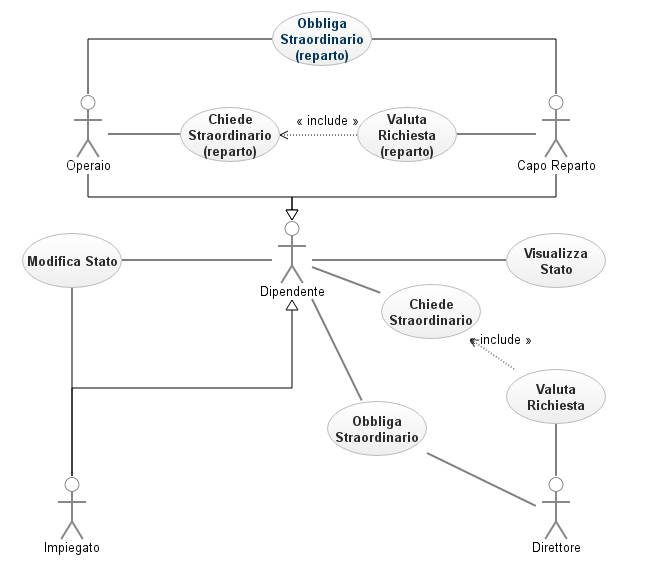
\includegraphics[scale=0.7]{use-case}}} \\
	\hline
	\end{tabular}
	\end{table}
	\FloatBarrier

	%.............................................................

	\FloatBarrier
	\begin{table}[h|]
	\centering
	\begin{tabular}{p{3cm}p{11cm}}
	\textbf{Use case} & \textit{Chiede straordinario} \\ 
	\textbf{Attori} & Dipendente (iniziatore), Direttore \\ 
	\textbf{Tipo} & Primario \\ 
	\textbf{Descrizione} & Il dipendente inserisce una richiesta per effettuare ore di straordinario \\
	\\
	\end{tabular}
	\centering
	\begin{tabular}{|p{7cm}|p{7cm}|}
	\hline
	\textbf{Azione attore} & \textbf{Risposta del sistema} \\ \hline
	1. Il dipendente inserisce una richiesta per effettuare ore di straordinario &                  \\ \hline
	& 2. Il sistema verifica la validità della richiesta                  \\ \hline
	& 3. Il sistema inserisce la richiesta nel database                  \\ \hline
	& 4. Il sistema invia una notifica al direttore                  \\ \hline
	5. Il direttore verifica la richiesta del dipendente &                   \\ \hline
	\multicolumn{2}{|c|}{\textbf{Eccezioni}} \\ \hline
	\multicolumn{2}{|l|}{ 2. La data inserita risulta in un giorno di chiusura dell'azienda } \\ \hline
	\multicolumn{2}{|l|}{ 2. Il dipendente ha già raggiunto il massimo di ore di straordinario valide da contratto } \\ \hline
	\end{tabular}
	\end{table}
	\FloatBarrier
	
	%.............................................................
	
	\FloatBarrier
	\begin{table}[h|]
	\centering
	\begin{tabular}{p{3cm}p{11cm}}
	\textbf{Use case} & \textit{Chiede straordinario (reparto)} \\ 
	\textbf{Attori} & Operaio (iniziatore), Capo Reparto \\ 
	\textbf{Tipo} & Primario \\ 
	\textbf{Descrizione} & L'operaio inserisce una richiesta per effettuare ore di straordinario destinata al proprio capo reparto \\
	\\
	\end{tabular}
	\centering
	\begin{tabular}{|p{7cm}|p{7cm}|}
	\hline
	\textbf{Azione attore} & \textbf{Risposta del sistema} \\ \hline
	1. L'operaio inserisce una richiesta per effettuare ore di straordinario &                  \\ \hline
	& 2. Il sistema verifica la validità della richiesta                  \\ \hline
	& 3. Il sistema inserisce la richiesta nel database                  \\ \hline
	& 4. Il sistema invia una notifica al capo del reparto dell'operaio                  \\ \hline
	5. Il capo reparto verifica la richiesta del dipendente &                   \\ \hline
	\multicolumn{2}{|c|}{\textbf{Eccezioni}} \\ \hline
	\multicolumn{2}{|l|}{ 2. La data inserita risulta in un giorno di chiusura dell'azienda } \\ \hline
	\multicolumn{2}{|l|}{ 2. L'operaio ha già raggiunto il massimo di ore di straordinario valide da contratto } \\ \hline
	\end{tabular}
	\end{table}
	\FloatBarrier

	%.............................................................

	\FloatBarrier
	\begin{table}[h|]
	\centering
	\begin{tabular}{p{3cm}p{11cm}}
	\textbf{Use case} & \textit{Obbliga straordinario} \\ 
	\textbf{Attori} & Direttore (iniziatore), Dipendente \\
	\textbf{Tipo} & Primario \\
	\textbf{Descrizione} & Il direttore richiede ad un dipendente di effettuare ore di straordinario. \\
	\\
	\end{tabular}
	\centering
	\begin{tabular}{|p{7cm}|p{7cm}|}
	\hline
	\textbf{Azione attore} & \textbf{Risposta del sistema} \\ \hline
	1. Il direttore inserisce una richiesta effettuare ore di straordinario destinata ad uno specifico dipendente &                  \\ \hline
	& 2. Il sistema verifica la validità della richiesta                  \\ \hline
	& 3. Il sistema inserisce la richiesta nel database                  \\ \hline
	& 4. Il sistema invia una notifica al dipendente                  \\ \hline
	\multicolumn{2}{|c|}{\textbf{Eccezioni}} \\ \hline
	\multicolumn{2}{|l|}{ 2. La data inserita risulta in un giorno di chiusura dell'azienda } \\ \hline
	\multicolumn{2}{|l|}{ 2. Il dipendente ha già raggiunto il massimo di ore di straordinario valide da contratto } \\ \hline
	\end{tabular}
	\end{table}
	\FloatBarrier
	
	%.............................................................

	\FloatBarrier
	\begin{table}[h|]
	\centering
	\begin{tabular}{p{3cm}p{11cm}}
	\textbf{Use case} & \textit{Obbliga straordinario (reparto)} \\ 
	\textbf{Attori} & Capo Reparto (iniziatore), Operaio \\
	\textbf{Tipo} & Primario \\
	\textbf{Descrizione} & Il capo reparto richiede ad un operaio di effettuare ore di straordinario. \\
	\\
	\end{tabular}
	\centering
	\begin{tabular}{|p{7cm}|p{7cm}|}
	\hline
	\textbf{Azione attore} & \textbf{Risposta del sistema} \\ \hline
	1. Il capo reparto inserisce una richiesta effettuare ore di straordinario destinata ad uno specifico operaio &                  \\ \hline
	& 2. Il sistema verifica la validità della richiesta                  \\ \hline
	& 3. Il sistema inserisce la richiesta nel database                  \\ \hline
	& 4. Il sistema invia una notifica all'operaio                  \\ \hline
	\multicolumn{2}{|c|}{\textbf{Eccezioni}} \\ \hline
	\multicolumn{2}{|l|}{ 2. La data inserita risulta in un giorno di chiusura dell'azienda } \\ \hline
	\multicolumn{2}{|l|}{ 2. L'operaio ha già raggiunto il massimo di ore di straordinario valide da contratto } \\ \hline
	\end{tabular}
	\end{table}
	\FloatBarrier

	%.............................................................

	\FloatBarrier
	\begin{table}[h|]
	\centering
	\begin{tabular}{p{3cm}p{11cm}}
	\textbf{Use case} & \textit{Valuta richiesta} \\ 
	\textbf{Attori} & Direttore (iniziatore), Dipendente \\ 
	\textbf{Tipo} & Primario \\ 
	\textbf{Descrizione} & Il direttore valuta una richiesta di straordinario di un dipendente \\
	\\
	\end{tabular}
	\centering
	\begin{tabular}{|p{7cm}|p{7cm}|}
	\hline
	\textbf{Azione attore} & \textbf{Risposta del sistema} \\ \hline
	1. Il direttore seleziona la richiesta ed inserisce la propria valutazione &                  \\ \hline
	 & 2. Il sistema memorizza la scelta \\ \hline
	& 3. Il sistema invia una notifica al dipendente\\ \hline
	\multicolumn{2}{|c|}{\textbf{Eccezioni}} \\ \hline
	\multicolumn{2}{|l|}{ - } \\ \hline
	\end{tabular}
	\end{table}
	\FloatBarrier
	
		\FloatBarrier
	\begin{table}[h|]
	\centering
	\begin{tabular}{p{3cm}p{11cm}}
	\textbf{Use case} & \textit {Valuta richiesta (reparto)} \\ 
	\textbf{Attori} & Capo Reparto (iniziatore), Operaio \\ 
	\textbf{Tipo} & Primario \\ 
	\textbf{Descrizione} & Un capo reparto valuta una richiesta di straordinario di un operaio\\
	\\
	\end{tabular}
	\centering
	\begin{tabular}{|p{7cm}|p{7cm}|}
	\hline
	\textbf{Azione attore} & \textbf{Risposta del sistema} \\ \hline
	1. Il capo reparto seleziona la richiesta ed inserisce la propria valutazione &                  \\ \hline
	 & 2. Il sistema memorizza la scelta \\ \hline
	& 3. Il sistema invia una notifica all'operaio\\ \hline
	\multicolumn{2}{|c|}{\textbf{Eccezioni}} \\ \hline
	\multicolumn{2}{|l|}{ - } \\ \hline
	\end{tabular}
	\end{table}
	\FloatBarrier
	
		\FloatBarrier
	\begin{table}[h|]
	\centering
	\begin{tabular}{p{3cm}p{11cm}}
	\textbf{Use case} & \textit{Visualizza stato} \\ 
	\textbf{Attori} & Dipendente (iniziatore) \\ 
	\textbf{Tipo} & Secondario \\ 
	\textbf{Descrizione} & Un dipendente visualizza la propria scheda \\
	\\
	\end{tabular}
	\centering
	\begin{tabular}{|p{7cm}|p{7cm}|}
	\hline
	\textbf{Azione attore} & \textbf{Risposta del sistema} \\ \hline
	1. Il dipendente inserisce le proprie credenziali di accesso &                  \\ \hline
	 & 2. Il sistema verifica le credenziali \\ \hline
	3. Il dipendente visualizza la propria scheda & \\ \hline
	\multicolumn{2}{|c|}{\textbf{Eccezioni}} \\ \hline
	\multicolumn{2}{|l|}{ 2. Le credenziali non sono corrette. } \\ \hline
	\end{tabular}
	\end{table}
	\FloatBarrier
	
	%.............................................................
	
	\FloatBarrier
	\begin{table}[h|]
	\centering
	\begin{tabular}{p{3cm}p{11cm}}
	\textbf{Use case} & \textit{Modifica stato} \\ 
	\textbf{Attori} & Impiegato (iniziatore), Dipendente \\ 
	\textbf{Tipo} & Primario \\ 
	\textbf{Descrizione} & Un impiegato modifica la situazione oraria e/o la scheda di un dipendente \\
	\\
	\end{tabular}
	\centering
	\begin{tabular}{|p{7cm}|p{7cm}|}
	\hline
	\textbf{Azione attore} & \textbf{Risposta del sistema} \\ \hline
	1. L'impiegato inserisce le proprie credenziali &                  \\ \hline
	& 2. Il sistema verifica le credenziali                  \\ \hline
	3. L'impiegato inserisce il codice del dipendente & \\ \hline
	& 4. Il sistema verifica il codice del dipendente                  \\ \hline
		5. L'impiegato modifica la situazione oraria e/o scheda del dipendente &                  \\ \hline
		& 6. Il sistema verifica i dati inseriti                  \\ \hline
	& 7. Il sistema visualizza la scheda del dipendende aggiornata                  \\ \hline
		8. Il dipendente riceve una notifica riguardo la modifica del proprio stato &                  \\ \hline
	\multicolumn{2}{|c|}{\textbf{Eccezioni}} \\ \hline
	\multicolumn{2}{|l|}{ 2. Le credenziali non sono corrette.} \\ \hline
		\multicolumn{2}{|l|}{ 4. Il codice del dipendente non è corretto.} \\ \hline
		\multicolumn{2}{|l|}{ 6. Si è verificato un errore nell'inserimento dei dati.} \\ \hline
	\end{tabular}
	\end{table}
	\FloatBarrier
	
%%%%%%%%%%%%%%%%%%%%%%%%%%%%%%%%%%%%%%%%%%%%%%%%%%%%%%%%%%%%%%%%%%%%%%%%

\FloatBarrier
\section{Diagramma delle attività}

	\hspace*{-0.8cm}
	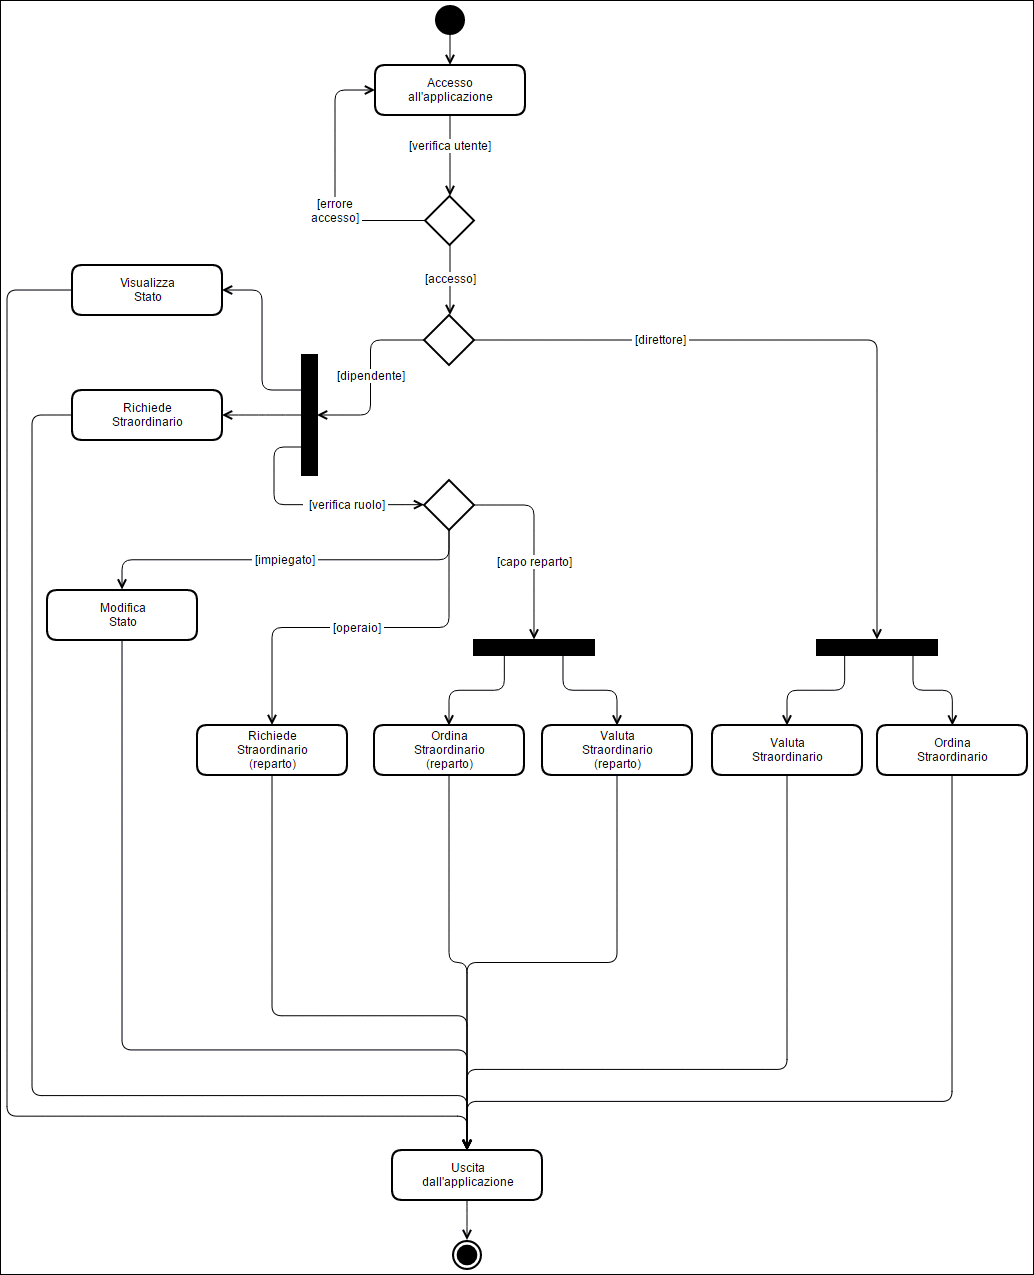
\includegraphics[scale=0.6]{activity}

%%%%%%%%%%%%%%%%%%%%%%%%%%%%%%%%%%%%%%%%%%%%%%%%%%%%%%%%%%%%%%%%%%%%%%%%

\pagebreak

\section{Diagramma delle classi}
	\FloatBarrier
	\begin{table}[h|]
	\hspace*{-1.70cm}
	\begin{tabular}{|c|}
	\hline
	{ \specialcell{ \\ 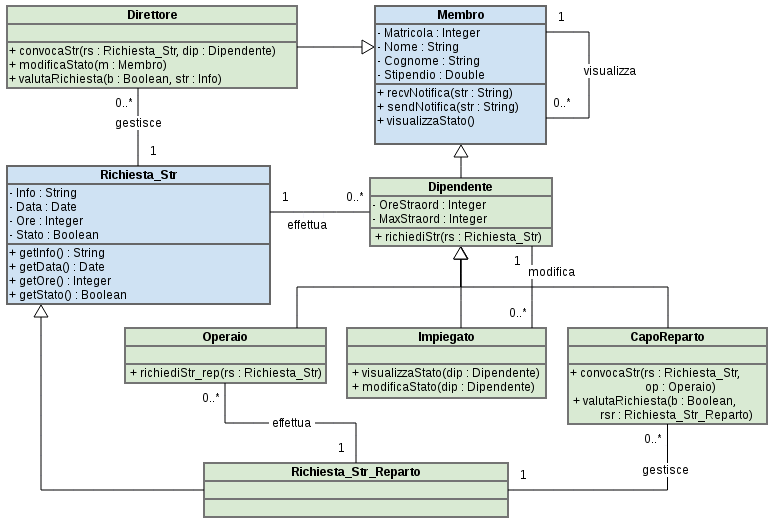
\includegraphics[scale=0.63]{classes}}} \\
	\hline
	\end{tabular}
	\end{table}
	\FloatBarrier

%%%%%%%%%%%%%%%%%%%%%%%%%%%%%%%%%%%%%%%%%%%%%%%%%%%%%%%%%%%%%%%%%%%%%%%%

\pagebreak

\section{Diagramma di sequenza}
	{\centering
	\specialcell{\\}
	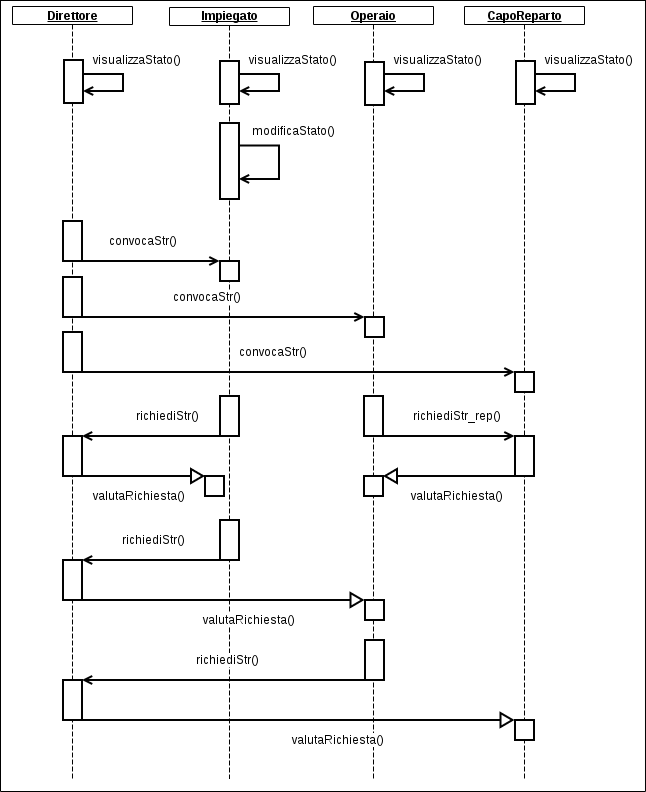
\includegraphics[scale=0.9]{sequence}\par
	}
%---------------------------------------------------------------------

\chapter{Design Patterns}
%Formato dei design pattern in stile GoF
%Nome e tipo:	-
%				-
%Scopo: 		che cosa fa il pattern e quando la soluzione è
%				applicabile e può portare benefici
%AKA:			altri nomi in uso per il pattern
%				-
%Motivazione:	problemi che sono stati risolti mediante
%				l’uso del pattern
%Applicabilità: situazioni dove il pattern
%				può essere applicato e può portare beneficio
%Struttura:		descrizione della soluzione, indica i partecipanti
%				e le collaborazioni
%Conseguenze:	vantaggi e svantaggi, trade-off e questioni che
%				nascono dall’impiego del pattern
%Implement:		suggerimenti e tecniche utili
%
%Utilizzi noti:	sistemi reali in cui il pattern è stato utilizzato
%				con successo
%Correlati:		-
%				-


I seguenti design pattern rappresentano soluzioni riusabili per trattare problemi ricorrenti nella realizzazione del prodotto.\\
Sono indipendenti dal linguaggio di programmazione utilizzato.
\subsection{Façade}
\section{Pattern strutturali}
Il pattern strutturale \textit{façade} si utilizza per offrire un’interfaccia uniforme ad un sotto-sistema complesso.\\
In questo caso si suggerisce l'applicazione di tale pattern all'interfaccia di richiesta degli straordinari.\\\\

	{\centering
	\hspace*{-2.23cm}
	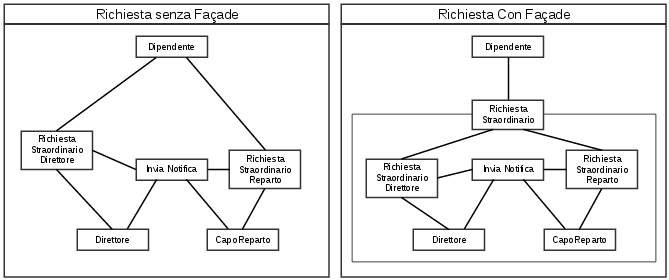
\includegraphics[scale=0.8]{facade}\par
	}

%---------------------------------------------------------------------

%\chapter{Appendici}
%Tutto ciò che può essere utile ma non è essenziale per specificare
%i requisiti (norme, convenzioni, supporti)
%Lorem ipsum dolor sit amet.

%%%%%%%%%%%%%%%%%%%%%%%%%%%%%%%%%%%%%%%%%%%%%%%%%%%%%%%%%%%%%%%%%%%%%

%Indice analitico

%\printindex
%Uso: Parola\index{parola}

\pagebreak
\blankpage{}

\end{document}
